\documentclass[withoutpreface]{cumcmthesis}
\usepackage{url} % 支持网址链接，便于引用网络资源
\usepackage{graphicx} % 插入和管理图片
\usepackage{pdflscape} % 使页面横向显示，适合宽表格
\usepackage{tabularx} % 支持自动调整宽度的表格
\usepackage{afterpage} % 控制内容在下一页显示
\usepackage{longtable} % 支持跨页长表格
\usepackage{booktabs}
\usepackage[numbers,sort&compress]{natbib} % 参考文献排序与压缩显示

\usepackage[figuresright]{rotating} % 支持图表旋转

\usepackage{needspace} % 控制内容在页面底部不被截断
\usepackage{amsmath} % 数学公式增强
\usepackage{amssymb} % 更多数学符号
\usepackage{geometry} % 页面边距自定义
\usepackage{enumitem} % 列表样式自定义
\usepackage{caption} % 图表标题样式自定义
\usepackage{fancyhdr} % 页眉页脚自定义
\usepackage{titlesec} % 章节标题样式自定义

\usepackage{listings} % 插入和高亮显示代码
\newfontfamily\codefont{DejaVu Sans Mono}
% 设置代码样式
\lstset{
	numbers             =   left,               % 行号显示在左侧
	showspaces          =   false,              % 不显示空格符号
	numberstyle         =   \zihao{-5}\codefont,% 行号风格，小五号，等宽字体
	showstringspaces    =   false,              % 不显示字符串中的空格
	captionpos          =   t,                  % 标题位置在顶部
	frame               =   lrtb,               % 显示四周边框
	breaklines          =   true,               % 自动换行
	columns             =   fixed,              % 固定列宽
	basewidth           =   0.5em,              % 基础宽度
	caption             =   \raggedright,       % 标题左对齐
	literate            =   {ρ}{{$\rho$}}1
	                        {σ}{{$\sigma$}}1
	                        {δ}{{$\delta$}}1
	                        {κ}{{$\kappa$}}1,    % 保证附录代码中的希腊字母可正确显示
}

% Python 代码样式
\lstdefinestyle{Python}{
	language        =   Python, % 语言设为Python
	basicstyle      =   \zihao{-5}\codefont\color{black}, % 基本风格，小五号，等宽字体，黑色
	keywordstyle    =   \color{blue}\bfseries\itshape, % 关键字风格，蓝色加粗斜体
	stringstyle     =   \color{magenta}, % 字符串风格，洋红色
	commentstyle    =   \color{red}\itshape, % 注释风格，红色斜体
}

% MATLAB 代码样式
\lstdefinestyle{MATLAB}{
	language        =   Matlab, % 语言设为MATLAB
	basicstyle      =   \zihao{-5}\codefont\color{black}, % 基本风格，小五号，等宽字体，黑色
	keywordstyle    =   \color{green}\bfseries\itshape, % 关键字风格，绿色加粗斜体
	stringstyle     =   \color{purple}, % 字符串风格，紫色
	commentstyle    =   \color{gray}\itshape, % 注释风格，绿色斜体
}



\usepackage{xcolor} % 颜色支持，代码和表格可用
\usepackage{multicol} % 多栏排版

\usepackage{booktabs} % 优美的表格线
\usepackage{hyperref} % 支持PDF跳转、超链接
\usepackage{subcaption} % 子图标题，多个图片并排显示
\usepackage {float}  % 更灵活地控制浮动体（如表格、图片）位置
\usepackage{array} % 增强表格功能
\hypersetup{hidelinks,
	colorlinks=true,
	allcolors=black,
	pdfstartview=Fit,
	breaklinks=true
}
\usepackage{siunitx} % 科学计数法和单位格式化
\usepackage{threeparttable}
\usepackage{placeins}
\usepackage{microtype}
\geometry{left=2.4cm,right=2.4cm,top=2.35cm,bottom=2.35cm}
\captionsetup{font=small,labelfont=bf}

\title{锂离子电池快充寿命的建模预测与策略优化研究}
\tihao{A}
\baominghao{}
%\schoolname{BIT}			%学校  
%\yearinput{2025}			%年份  
%\monthinput{09}			%月份
%\dayinput{03}				%日期

\begin{document}

\pagenumbering{arabic}

\maketitle
\begin{center}
    {\heiti\zihao{-4} 摘\quad 要}
\end{center}


\textbf{针对问题一},

\textbf{针对问题二},

\textbf{针对问题三},

\textbf{针对问题四},

\noindent\textbf{关键词：}


\clearpage

\section{问题重述}
\subsection{问题背景}
干燥是决定中药材品质的核心工序，其中热风烘干是常见的干燥方式之一。该方式主要包括预热平衡和恒温干燥两个阶段，通过调节烘房温湿度，得到干燥药材。在中药材烘干时，不当的工艺参数选取易导致干燥效率低、能耗高、品质不稳定等缺陷。而传统的试验优化模式存在周期长、成本高等问题，需要借助数理方法与仿真得到干燥规律。
\subsection{问题提出}
\textbf{问题一:}根据药材初始状态、烘房环境变化以及题目给定的传热传质参数，研究烘干预热阶段药材内部温度和水分浓度随时间及径向位置的变化规律，并计算题目指定时刻和位置对应的温度与水分浓度。

\textbf{问题二:}将研究范围扩展至完整烘干过程，考虑药材密度、比热容、导热系数以及水分扩散能力随温度和含水率发生变化，描述药材内部温度和水分浓度的动态变化，并给出烘干前 3 小时指定时刻和位置的温湿状态。

\textbf{问题三:}在完整烘干过程的基础上，以药材内部各位置的水分浓度均低于 \(0.15\,\mathrm{kg/kg}\) 作为干燥要求，研究药材内部水分随时间的变化，并确定满足该要求所需要的烘干时间。

\textbf{问题四:}进一步考虑药材在失水过程中发生的尺寸收缩，结合附件给出的半径随时间变化数据以及相应的材料物性关系，研究尺寸变化条件下药材内部水分浓度的变化，并重新确定药材达到规定干燥要求所需的时间。




\section{问题分析}
\subsection{问题一分析}
问题一研究药材在烘干初始阶段内部温度和水分浓度的变化。烘房温度和水分浓度随时间变化，使药材与外界之间产生温度差和水分差，进而引起热量传递和水分迁移。由于热量和水分从药材表面逐渐向内部传递，不同位置对外界环境变化的响应存在差异，因此需要同时考虑时间和空间对温度、水分分布的影响。此外，药材呈有限长度的圆柱形，传递过程可能受到径向、轴向及端部作用的影响，其几何尺寸、传热传质性质和表面交换条件均会影响内部温湿状态的变化。
\subsection{问题二分析}
问题二将研究范围扩展至整个烘干过程。随着水分不断排出，药材自身的传热传质性质也随之变化。题目给出的经验关系表明，密度、比热容和导热系数受到含水率影响，而水分扩散能力又同时受到温度和含水率影响。因此，含水率变化会改变药材的传热特性，温度变化又会影响水分迁移速度，使温度、水分和材料物性之间形成相互影响的动态过程。由此需要在问题一的基础上进一步描述物性不断变化情况下药材整个烘干过程中的温湿变化。
\subsection{问题三分析}
问题三要求确定药材达到规定干燥程度所需的时间。由于题目要求药材所有位置的水分浓度均低于 \(0.15\,\mathrm{kg/kg}\)，因此不能仅依据表面或平均水分浓度判断烘干完成，而需要关注整个药材内部水分浓度较高、干燥较慢的位置。随着烘干持续进行，不同位置的失水速度以及水分扩散能力均会发生变化，因此需要在全过程温湿变化的基础上持续考察药材内部水分分布，从而确定整体满足干燥要求的时刻。
\subsection{问题四分析}
问题四进一步考虑失水引起的药材尺寸变化。附件2表明药材半径随烘干时间逐渐减小，使药材的边界位置以及内部热量和水分的传递距离随时间发生变化；与此同时，本问给出的密度、比热容、导热系数和水分扩散能力也会随内部状态改变。因此，该问题需要综合考虑外界温湿环境、材料物性变化以及几何收缩对传热传质过程的共同影响，描述尺寸不断变化情况下药材内部水分的迁移过程，并进一步确定达到规定干燥要求所需的时间。
\section{模型假设}
为了对问题进行简化分析，本文在建立模型时作出如下假设：
\begin{enumerate}[label=(\arabic*)]
    \item 药材为均质各向同性材料，且在烘干过程中不发生化学反应。
    \item 药材的初始温度和水分浓度在整个体积内均匀分布。
    \item 干燥过程中药材所处环境的温度、湿度和烘干气体流速保持恒定。
    \item 药材水分迁移至表面后快速散失，且不考虑蒸发对药材温度影响。
    \item 
\end{enumerate}
\section{主要符号说明}
\begin{table}[H]
\centering
\caption{主要符号及含义}
\label{tab:main_symbols}
\small
\setlength{\tabcolsep}{2pt}
{ 
\renewcommand{\arraystretch}{0.95} 
\begin{tabularx}{\textwidth}{cXcX}
\toprule
符号 & 含义 & 符号 & 含义 \\
\midrule


\bottomrule
\end{tabularx}
}
\end{table}
\section{模型的建立与求解}

\subsection{问题一：}
\section{问题1的模型建立}\label{sec:q1model}
依据上一章的模型假设，本章把药材预热过程表述为一维径向初边值问题：先确定空间范围与状态变量，再由热量、水分守恒建立控制方程，最后配置初值和边界条件。完整模型交由第\ref{sec:q1solve}章求解，其数值精度及一维简化的适用性统一在第\ref{sec:q1check}章检验。图\ref{fig:flow}给出这一论述顺序。
\begin{figure}[H]\centering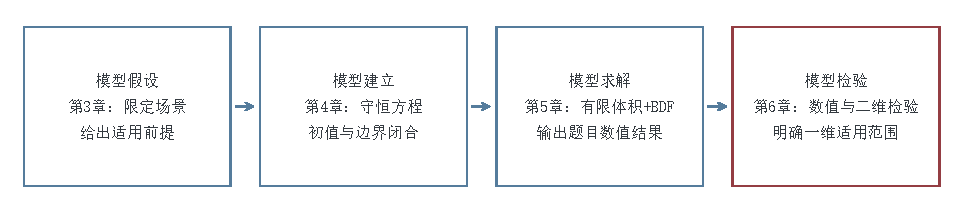
\includegraphics[width=\textwidth]{figures/q1_flowchart.pdf}
\caption{问题1的建模论证逻辑}\label{fig:flow}
\end{figure}
\Needspace{7\baselineskip}
\subsection{建模对象与径向抽象}
题给药材半径$R=0.02$~m、全长$L=0.25$~m，半长$H=L/2=0.125$~m。取单位轴向长度的药材截面，径向范围为$0\le r\le R$，待求状态为温度$\theta_1(r,t)$与干基含水率$C_1(r,t)$。外界变化通过侧面对流换热和水分交换传入材料，内部状态随半径变化。因此，一维模型保留径向梯度，并不将药材视为整体均匀的集中参数系统。

图\ref{fig:radial}左侧标出从轴心$O$到侧面$S$的径向测量线，右侧标出用于守恒分析的环形微元。此处忽略轴向输运与端面交换，以预测中截面附近的局部状态；这是一项待检验的近似，不能提前推广到整个圆柱。
\begin{figure}[H]\centering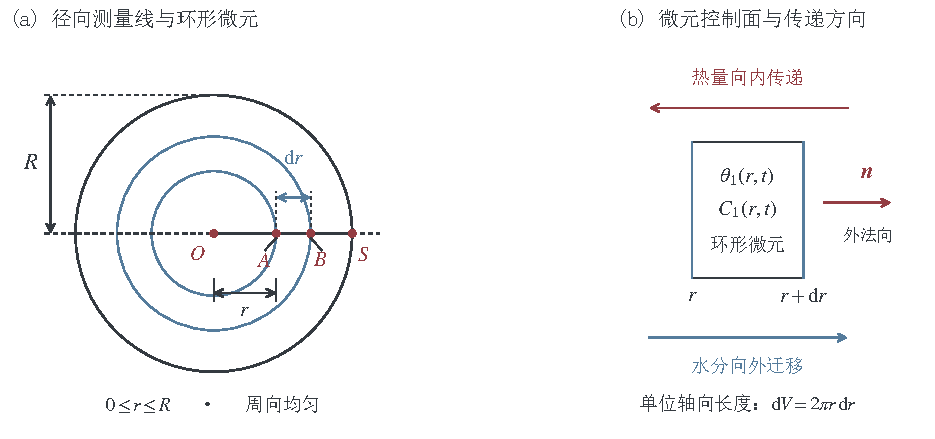
\includegraphics[width=\textwidth]{figures/q1_radial_geometry.pdf}
\caption{径向测量线与环形微元}\label{fig:radial}
\end{figure}
\subsection{温度控制方程}

本问采用附录2给定的密度
$\rho=820$\~kg/m$^3$、比热容
$c_p=2600$\~J/(kg$\cdot$K)、
热传导系数
$k=0.36$\~W/(m$\cdot$K)。
本文温度统一采用摄氏温度$\theta$表示。由于摄氏温标与热力学温标仅相差常数$273.15$，二者的温度变化量及空间、时间导数完全相同，因此不影响下述传热方程的建立。

取药材中半径为$r$、径向厚度为$dr$的单位轴向长度环形微元。其体积为
\[
dV
=
\pi\left[(r+dr)^2-r^2\right]\times1
=
\pi(2r\,dr+dr^2).
\]
当$dr$足够小时，二阶小量$dr^2$相对于$dr$可忽略，因此
\[
dV\approx2\pi r\,dr.
\]

设药材温度为$\theta_1(r,t)$。微元质量为
\[
dm=\rho\,dV,
\]
温度发生微小变化$d\theta_1$时，其显热变化为
\[
dQ=dm\,c_p\,d\theta_1
=\rho c_p dV\,d\theta_1.
\]
因此单位时间内微元的储热变化率为
\[
\frac{dQ}{dt}
=
\rho c_p(2\pi r\,dr)
\frac{\partial\theta_1}{\partial t}.
\]

另一方面，记$q_r(r,t)$为沿径向向外取正的热流密度，单位为W/m$^2$。在微元内侧$r$处，传热面积为$2\pi r$，对应的径向热流率为
\[
2\pi r\,q_r(r,t).
\]
在外侧$r+dr$处，热流率为
\[
2\pi(r+dr)\,q_r(r+dr,t).
\]
因此，微元的净热流入为
\[
2\pi r\,q_r(r,t)
-
2\pi(r+dr)\,q_r(r+dr,t).
\]
对外侧热流率作一阶展开，
\[
2\pi(r+dr)q_r(r+dr,t)
\approx
2\pi rq_r(r,t)
+
\frac{\partial}{\partial r}
\left(2\pi rq_r\right)dr,
\]
故净热流入可写为
\[
-\frac{\partial}{\partial r}
\left(2\pi rq_r\right)dr.
\]

根据能量守恒，微元的储热变化率应等于净热流入，即
\[
\rho c_p(2\pi r\,dr)
\frac{\partial\theta_1}{\partial t}
=
-\frac{\partial}{\partial r}
\left(2\pi rq_r\right)dr.
\]

再由傅里叶定律，
\[
q_r
=
-k\frac{\partial\theta_1}{\partial r}.
\]
其中，当温度沿径向向外升高时，
$\partial_r\theta_1>0$，则$q_r<0$，表示实际热量向内传递，与预热过程的物理情况一致。

将傅里叶定律代入能量守恒式，并约去公共因子$2\pi\,dr$，得到
\[
\rho c_p r
\frac{\partial\theta_1}{\partial t}
=
\frac{\partial}{\partial r}
\left(
kr\frac{\partial\theta_1}{\partial r}
\right).
\]
由于本问中$k$、$\rho$、$c_p$均为常数，可进一步写为
\begin{equation}
\frac{\partial\theta_1}{\partial t}
=
\alpha\frac1r
\frac{\partial}{\partial r}
\left(
r\frac{\partial\theta_1}{\partial r}
\right),
\qquad
\alpha=\frac{k}{\rho c_p}.
\label{eq:heat1}
\end{equation}

式\eqref{eq:heat1}描述药材内部沿径向的显热传导过程。该式建立在物性参数恒定、无体积热源且不考虑相变潜热等假设之上。
\subsection{水分控制方程}

药材干基含水率$C_1(r,t)$定义为水分质量与干物质质量之比。在恒定干物质密度$\rho_d$条件下，单位体积内所含水分质量为
\[
\rho_d C_1.
\]

仍取半径为$r$、径向厚度为$dr$的单位轴向长度环形微元，其体积近似为
\[
dV=2\pi r\,dr.
\]
因此微元中的水分质量为
\[
dm_w
=
\rho_d C_1\,dV
=
\rho_d C_1(2\pi r\,dr).
\]
单位时间内该微元水分储量的变化率为
\[
\frac{dm_w}{dt}
=
\rho_d(2\pi r\,dr)
\frac{\partial C_1}{\partial t}.
\]

记$J_r(r,t)$为沿径向向外取正的水分质量通量，单位为kg/(m$^2\cdot$s)。根据有效Fick定律，
\[
J_r
=
-\rho_dD(C_1)
\frac{\partial C_1}{\partial r}.
\]

在内侧$r$处，水分流率为
\[
2\pi rJ_r(r,t),
\]
在外侧$r+dr$处，水分流率为
\[
2\pi(r+dr)J_r(r+dr,t).
\]
因此微元的净水分流入为
\[
-\frac{\partial}{\partial r}
\left(2\pi rJ_r\right)dr.
\]

由水分质量守恒，
\[
\rho_d(2\pi r\,dr)
\frac{\partial C_1}{\partial t}
=
-\frac{\partial}{\partial r}
\left(2\pi rJ_r\right)dr.
\]
代入Fick定律并约去公共因子$\rho_d$与$2\pi\,dr$，得到
\begin{equation}
\frac{\partial C_1}{\partial t}
=
\frac1r\frac{\partial}{\partial r}
\left[
rD(C_1)\frac{\partial C_1}{\partial r}
\right],
\qquad
D(C_1)=D_0\exp(-b/C_1).
\label{eq:moist1}
\end{equation}

式中
$D_0=7\times10^{-9}$\~m$^2$/s、
$b=0.89$\~kg/kg。
由于$D$随局部含水率$C_1$变化，因此不能将$D(C_1)$直接移到散度算子之外，否则会遗漏扩散系数空间变化对水分迁移的影响。
\subsection{初值、边界条件与模型闭合}

题给药材初始温度和含水率在空间上均匀，因此
\[
\theta_1(r,0)=28,
\qquad
C_1(r,0)=2.55.
\]

在轴心$r=0$处，由轴对称性可知不存在净径向热量与水分通量，因此满足
\[
\partial_r\theta_1(0,t)=0,
\qquad
\partial_rC_1(0,t)=0.
\]

在真实侧面$r=R$处，药材与外界环境之间分别通过对流换热和水分交换传递热量与水分，因此采用Robin边界条件。完整初边值条件为
\begin{equation}
\left\{
\begin{aligned}
\theta_1(r,0)&=28,
\qquad
C_1(r,0)=2.55,\\
\partial_r\theta_1(0,t)&=0,
\qquad
\partial_rC_1(0,t)=0,\\
-k\partial_r\theta_1(R,t)
&=
h[\theta_1(R,t)-\theta_\infty(t)],\\
-D(C_1)\partial_rC_1(R,t)
&=
h_m[C_1(R,t)-C_\infty(t)].
\end{aligned}
\right.
\label{eq:boundary1}
\end{equation}

取
$h=25$\~W/(m$^2\cdot$K)、
$h_m=8\times10^{-7}$\~m/s。
边界函数$\theta_\infty(t)$与$C_\infty(t)$由附件1中的环境记录采用分段线性插值得到。

外法向取径向向外。当环境温度高于药材表面温度时，
\[
\theta_\infty(t)>\theta_1(R,t),
\]
则
\[
h[\theta_1(R,t)-\theta_\infty(t)]<0,
\]
说明外向热通量为负，即实际热量由环境进入药材。另一方面，当药材表面含水率高于环境含水率时，
\[
C_1(R,t)>C_\infty(t),
\]
对应外向水分通量为正，即水分由药材向环境迁移。

因此，Robin边界条件确定的是药材表面与环境之间的交换通量，而不是直接令药材表面状态等于环境状态。

至此，式\eqref{eq:heat1}、式\eqref{eq:moist1}与式\eqref{eq:boundary1}共同构成问题1的一维径向传热传质模型。题给物性参数与环境记录作为模型输入，$\theta_1(r,t)$与$C_1(r,t)$为待求状态变量。

\subsection{问题二：}


\subsection{问题三：}




\subsection{问题四：}



\section{模型检验、误差与敏感性分析}


\section{模型评价与推广}



\section*{AI工具使用声明}
本参赛队在竞赛过程中使用了AI工具，主要用于代码框架生成与调试、统计分析方案讨论、图表排版、论文结构检查及语言润色。AI未用于生成、补造或修改实验数据；所有程序均由参赛队在本地环境运行，核心数据口径、模型选择、公式、数值结果、图表和结论均经人工审查与复核。详细工具型号、使用环节、提示方式、采纳修改及核验情况见支撑材料《AI工具使用详情.pdf》。

\addcontentsline{toc}{section}{参考文献}
\begingroup
\small
\bibliographystyle{unsrt}
\bibliography{book}
\endgroup


\clearpage
\appendix
\section{支撑材料文件列表}




\section{程序复现说明}

\clearpage
\section{关键源程序代码（节选）}




\end{document}
